Qt is a framework that streamlines the development of high-performance, visually appealing and feature-rich GUI applications. 
It offers support for multiple languages such as C++, Python, and JavaScript, so developers can choose their preferred language.
Thanks to the documentation and the large user base, it also has a lot of support material to look up \cite{qt}.

With the \hyperref[sub:qt_designer]{Qt Designer}, developers can create GUI designs effortlessly.
Designs can be created through drag-and-drop, which accelerates designing in Qt. 
It also enables developers to visualize what their application will look like in real-time \cite{qt}.

The feature-rich and vast knowledge base, coupled with its user-friendly design, made it 
an easy choice to use in this project to develop the applications.


\section{Qt Designer}
\label{sub:qt_designer}

This is a tool from the Qt framework that allows designing and building your GUI via drag-and-drop. 
It uses the what-you-see-is-what-you-get approach, where how it looks in the designer will be the 
same in the real application \cite{qt}.

In figure \ref{fig:qt_designer}, the Qt Designer application is shown. There, you have your main 
window where you can drag widgets from the left into it to place them in the application. If you 
select a layout for your widgets, Qt will automatically fit them according to the layout, so the 
developer knows the widgets will be aligned properly. In applications, it is important to know the 
hierarchy of the widgets. Qt Designer makes this an easy process to figure out. With the object 
window (on the top right), you can easily find out which widget is in which widget. To place a 
widget into another widget, it is as simple as dragging the widget into the other one. Not only 
can the content and placement of the widgets be adjusted, but you can also set multiple parameters 
of these widgets within Qt Designer (on the bottom right). This helps to instantly see the changes you made without 
starting your GUI application. This is really useful when changing the styles or the layout of 
certain widgets. These changes will be instantly represented in the Designer, so you don't have 
to guess how your application will look.

Qt Designer makes Qt an attractive choice for developers looking to create a GUI application. 
The real-time visualization makes creating a GUI easy and efficient, allowing you to try different 
looks of the application, resulting in a modern-looking design with minimal effort.

\begin{figure}
    \centering
    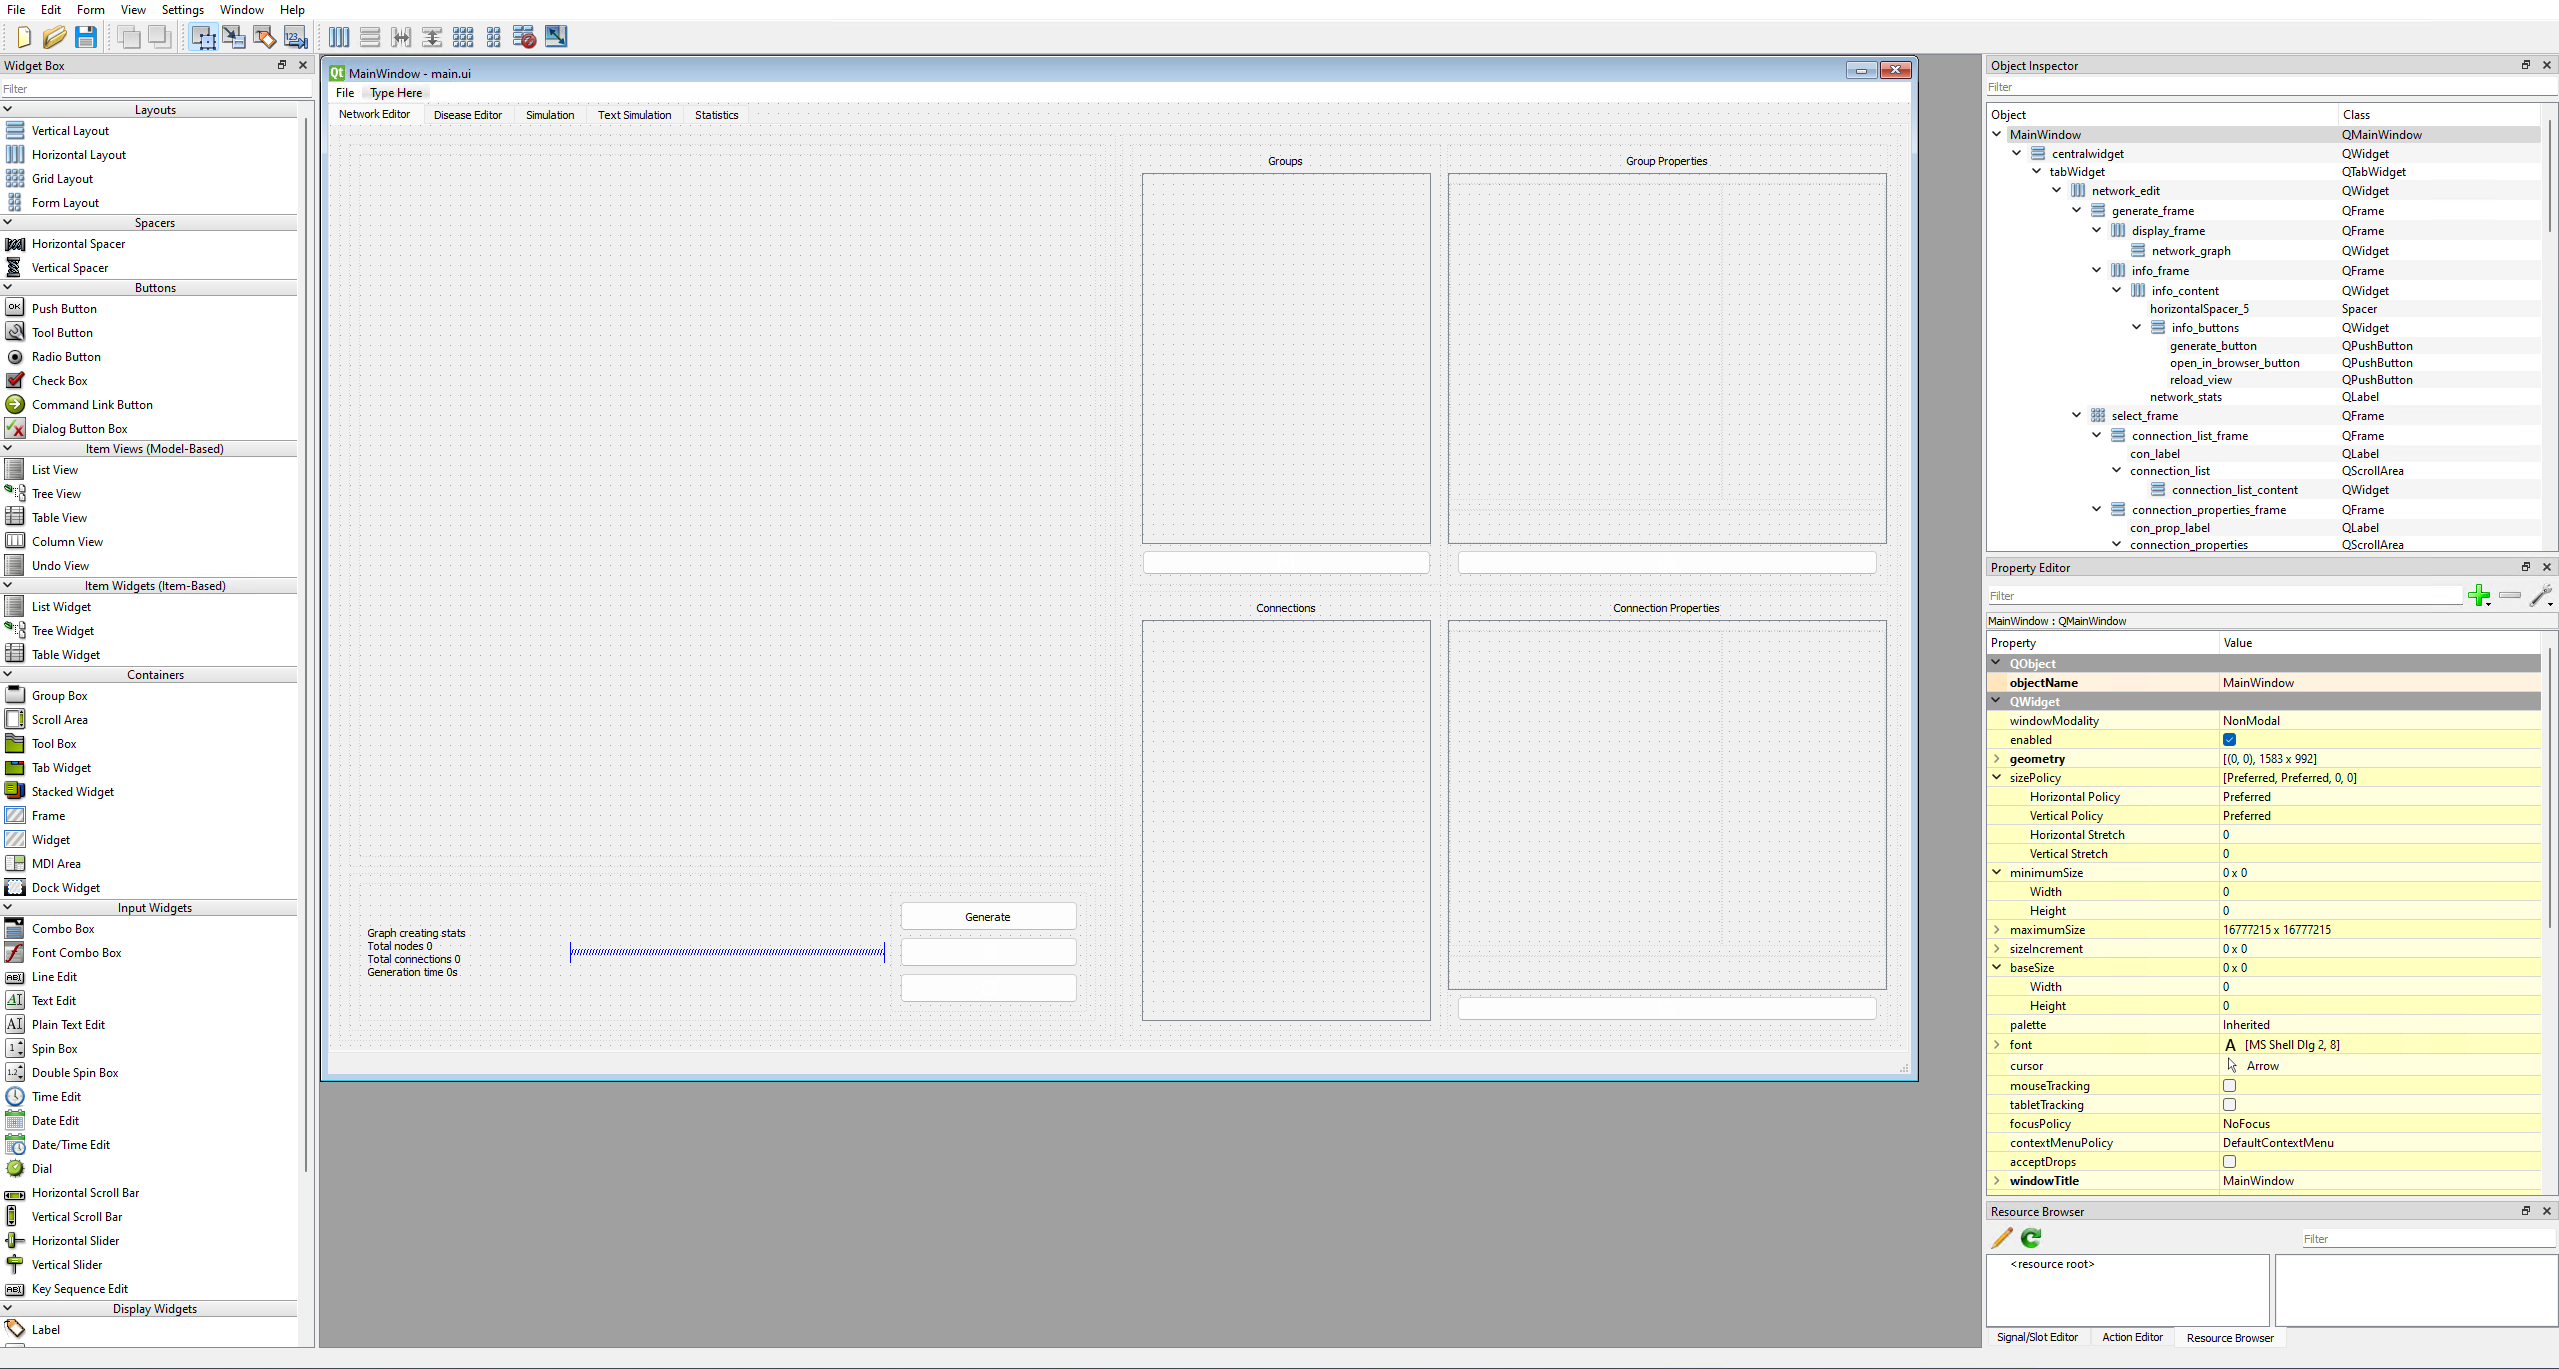
\includegraphics[width=0.8\linewidth]{images/qt_designer.png}
    \caption{Qt Designer}
    \label{fig:qt_designer}
\end{figure}

\section{PyQt}
\label{sub:pyqt}


Qt supports multiple programming languages to allow developers to choose their preferred language. 
This project was developed in Python; therefore, PyQt was used. PyQt is a module that can be easily 
installed via pip into the Python environment. It contains all the add-ons the C++ variant of Qt also has. 
The add-ons can be used by importing the corresponding Python module. To develop an application in PyQt, you can either 
create one by hand with only the Python commands or with the help of the Qt Designer. The GUI created in the 
Qt Designer is saved in a file that can be loaded in the PyQt application \cite{pyqt}. 
In listing \ref{lst:pyqt_gui}, it is shown how the design can be loaded into a simple application. 
If a design was loaded into the application, it makes it simple to access widgets that were 
created in the Qt Designer. To change widgets created in the Qt Designer, it is as simple as in line 7. 
The widget created in the Qt Designer was called \textit{myLabel}. Depending on what kind 
of widget it is, different functions are available. On a label, it is possible to change the text with 
\textit{setText}, but on a frame widget where no text is shown, it is not possible. If a design was loaded in, 
it is possible to add more widgets into it. For example, if buttons need to be created dynamically. This allows 
developers to create the default design of their application in the Qt Designer and change the contents or 
arrangement of the widgets in the application dynamically. The ease of access to the objects created by the 
Qt Designer helps to improve readability and simplicity in the application code.

\begin{lstlisting}[language=python, caption={Simple Qt GUI application}, label={lst:pyqt_gui}]
from PyQt5 import QtWidgets, uic
import sys
class GuiApplication(QtWidgets.QMainWindow):
    def __init__(self):
        super(GuiApplication, self).__init__()
        uic.loadUi('basic.ui', self)
        self.myLabel.setText('Changed text')
        self.show()

app = QtWidgets.QApplication(sys.argv)
window = GuiApplication()
app.exec_()
\end{lstlisting}

\section{Signals and Slots}
\label{sub:signals}

In GUI programming, it is often necessary to execute functions if, for example, a button is pressed. Other frameworks 
use callbacks to achieve this functionality; Qt uses the Signals and Slots mechanism. The signal is emitted by an 
object if its internal state changes. The slot is the function that will be executed once the signal is 
emitted. A signal can have multiple slots connected to it that will be executed one after the other. 
The Signal-Slot mechanism is independent of the GUI event loop and will be executed immediately after 
the signal is emitted \cite{qt}.

In order to connect a signal to a slot in PyQt, you have to call the \textit{.connect} function of a signal. 
For example, a button in Qt has three signals: \textit{clicked}, \textit{pressed}, and \textit{released}. 
In order to connect a function to the button, the command would look like \textit{example\_button.clicked.connect(slot\_function)}. 
Now, if the button is clicked by the user in the GUI, the \textit{slot\_function} will be executed \cite{pyqt}.

\subsection{Thread communication}
\label{sub:thread_communication}

In general, it is bad practice to have a thread modify widgets of the GUI to ensure the separation of concerns. 
If that thread were killed early, it could lead to an unexpected GUI state that can result in errors. Or if the 
main thread changed the structure of the GUI widgets before the thread could add the desired widgets, which would 
also lead to errors. To solve this issue, the Signals and Slots mechanism is ideal for that situation. Instead of 
letting the thread handle the widget creation, you have the thread send the data of the widget back to the main thread 
and let the main thread add or modify its widgets. That way, the integrity of the GUI can be maintained, as the 
main thread retains control over widget manipulation, ensuring consistent and expected behavior \cite{qt}.

In listing \ref{lst:pyqt_thread_comm}, a simple thread is displayed. It has two signals: the finished signal 
and the result signal. The result signal has a string as a parameter that will be sent along with the signal 
to the slot that will be executed. If the thread were to create a string that a label should have, it creates 
this string and emits it with the result signal. That way, the widget modification is only executed in the main 
thread and they are successfully separated \cite{pyqt}.

\begin{lstlisting}[language=python, caption={Thread example}, label={lst:pyqt_thread_comm}]
import sys
import time
from PyQt5.QtCore import pyqtSignal, QThread
class Worker(QThread):
    finished = pyqtSignal()
    result = pyqtSignal(str)

    def __init__(self):
        super().__init__()

    def run(self):
        time.sleep(2)
        result_data = "My Custom Data"
        self.result.emit(result_data)
        self.finished.emit()
\end{lstlisting}


\section{Abblication views}
\label{sub:thread_views}
In our GUI application, we have five tabs/views, each with a different use, simulating a spreading disease within a network.
\begin{description}
    \item[Network Editor] In this view, a user can create its network and the connections and view it in a 3D space.
    \item[Disease Editor] Here, diseases can be added that will be simulated spreading through the network.
    \item[Simulation] The Simulation view shows the website to simulate the disease's behavior in the network.
    \item[Text Simulation] If the network is too big, such that in the visual simulation would not be beneficial, it can be simulated just by showing text.
    \item[Statistics] This view helps analyze the result of a simulation.
\end{description}